\documentclass[conference,a4paper]{IEEEtran}

\usepackage{amsmath,amssymb,amsfonts}
\usepackage{graphicx}
\usepackage{textcomp}
\usepackage{xcolor}
\usepackage{booktabs}
\usepackage{array}
\usepackage{listings}
\usepackage{url}
\usepackage{hyperref}
\usepackage{cite}

\lstset{
	basicstyle=\ttfamily\footnotesize,
	keywordstyle=\color{blue}\bfseries,
	commentstyle=\color{gray}\itshape,
	stringstyle=\color{red},
	numbers=left,
	numberstyle=\tiny\color{gray},
	numbersep=5pt,
	frame=single,
	breaklines=true,
	captionpos=b,
	tabsize=4
}


\begin{document}

\title{Virtual Machines vs. Containers: A Performance Benchmark under WSL2}

\maketitle

\begin{abstract}
\mdseries This paper investigates how fast a Docker container is setup compared to a Virtual Machine running under the same application, and how they differ in memory, disk use and web performance. The main focus is actually the differences with the WSL2 environment in consideration, and seeing if the differences are still substantial. The study is made on a local device and requires no cloud account. I built one small Flask web service and ran it in two ways inside Windows Subsystem for Linux 2, one in a QEMU Virtual Machine with KVM acceleration, and another in a Docker container. Both were limited to two processor cores, and two gigabytes of memory. I measured the setup time, idle memory, disk size, throughput, and latency using ApacheBench with twenty thousand requests and fifty concurrent connections, while also repeating every measurement three times to ensure confidence in results. The container was ready in 0.77 seconds compared to the crazy 7.34 seconds for the virtual machine, used about 42 megabytes of memory compared to 522 megabytes, and took 212 megabytes of disk compared to 2334 megabytes. It also was able to serve around 33 percent more requests per second on a processer bound endpoint, and about twice as many on a lightweight endpoint. The study cost zero dollars, of course not considering the uptime costs of my machine as it took a lot of time to finish some runs. Results come from thee runs on one nested setup, so the difference is not a general ranking under Linux Virtual Machines, but rather on Nested ones (WSL2 in this scenario). For fast scaling of a stateless service the container is most definitely the better option, while the virtual machine is still good for when strong isolation is needed.
\end{abstract}

\begin{IEEEkeywords}
WSL2, Docker, containers, virtualisation, cloud computing
\end{IEEEkeywords}

\section{Introduction}
\label{sec:introduction}
Many people and even some organisations rely on WSL2 for their development environment, and many of them that run web services in the cloud need to decide on how to package them. A Virtual Machine image contains a complete operating system with its own kernel (all the settings, configurations, and dependencies) whereas a container image contains only the specific application and its user libraries and relies on the kernel of the host. Both approaches isolate the application from its surroundings, but they have very different behaviours in reality. The packaging choice affects how quickly the capacity expands when the userbase grows, how many instances of them fit on one server, how much storage images consume, and how much each running instance costs.

Those measurements are incredibly important for autoscaling. In autoscaling, noticing the traffic spike can only help new instances when they’re ready, so the time between the decision to scale out and the first served requests will determine how well the system handles load. If the starting instance takes several seconds, the system must either accept a period of lowered service, or supply enough alternative service. Containers start faster and are lighter than virtual machines ~\cite{b1,b2}, but the gap size actually depends on what is being run, on the hypervisor, environment (WSL2 for example), so it is worth measuring for a concrete case.

The scope of this study is extremely specific, I only compare two ways of running one application on one machine, I don’t compare cloud providers or instance types, or orchestration systems such as Kubernetes. Even though the contribution is small, it’s surely helpful in the specific extent, and is a completely scripted benchmark that reports startup time. memory, disk size, and web performance side by side, alongside the spread over repeated runs, so that anyone try my tests and judge based on their environment runs. The script, raw outputs, figures, and configuration files are available in the repository listed in the appendix.

The question(s) I’ve been following: On one host in the same application and same Ubuntu version and userspace, and the same budget of two CPU cores and two gigabytes of memory, (a) how fast is a Docker setup compared to a QEMU/KVM virtual machine, (b) how much memory and disk space does each one use, (c) is there a difference in throughput and response time (all considering the WSL2 environment)? I kept the application and system identical so that the differences we see are actually about the packaging and virtualisation approach, instead of the workload.

I deployed the same Flask service in both configurations and benchmarked each of them three times, with a script that shuffles target order per run to ensure effective testing. Everything ran on one WSL2 desktop, so the cost is only the runtime of the machine. Section~\ref{sec:related_work} covers related work, Section~\ref{sec:design} covers the design, Section~\ref{sec:methodology} covers the method, Section~\ref{sec:results} covers the results, and Sections~\ref{sec:discussion} and~\ref{sec:conclusion} cover the discussion and conclusion.

\section{Background and Related Work}
\label{sec:related_work}
Cloud computing provides an on-demand access to a bunch of resources, the NIST definition lists info about it such as resource pooling and rapid elasticity~\cite{b1}. Cloud computing also distinguishes infrastructure, platform, and Software as a Service (SaaS), and usually speaking, the Virtual Machines are the main part of Infrastructures as a Service (IaaS). The hypervisor presents virtual hardware to the operating system, which then boots its own kernel~\cite{b2}, and they’re usually grouped into two types: type 1 runs directly on the hardware, and type 2 runs as a program on a host operating system rather than a guest operating system~\cite{b2}.

Windows itself runs WSL2 on a lightweight Virtual Machine, so making a KVM guest launched from WSL2 would make it a nested Virtual Machine. The Linux kernel uses the KVM to act as the hypervisor in my setup, and QEMU provides the emulated devices and machine definition in user space~\cite{b5}. I have to specifically say that the nested Virtual Machine is not a hindrance, it is the main focus of this study, as both the container and Virtual Machine targets are tested in this environment. So any additional virtualisation is a key limitation to consider when trying to understand the results.

A Linux container is a normal process where the system view is restricted by kernel namespaces, and where the source use is limited with control groups (cgroups). All containers within the same host share the same kernel, so no extra kernel needs to boot, which makes this lightweight. But this also means a kernel vulnerability can compromise both the container and the host. Regardless, Docker exposes the limits as options: \texttt{--memory} caps memory use and \texttt{--cpuset-cpus} pins the container to specific cores~\cite{b4}.  We use both of these flags/options to set the budget (or hardware restrictions) to be the same as the Virtual Machine.

Rapid elasticity means that capacity can be provisioned and released quickly in response to demand~\cite{b1}. In real-world cases, the speed of this stretching and shrinking depends on the unit being scaled, and scaling in Virtual Machines basically means creating a machine, booting an operating system, and starting the application. Whereas scaling in containers means starting a process on a host that is already running. This is the reason that setup time is an actually useful metric for autoscaling and why I measure it in this report from the start command to the first successful HTTP response, and not only until a process exists.

Felter et al.~\cite{b3} has already made similar work, as they compared native Linux, KVM virtual machines, and Docker containers on processor, memory, network, and storage workload. In their work they’ve found that containers add almost no overhead for processor and memory related work and that virtualised networking is what has noticable consequences and issues. However, a gap in their study is the lack of information regarding how long the instances take to become ready, which is the first question of my work, which also used well known server benchmarks on Linux hardware. I instead measure a small Flask web service, report startup time, memory, and disk footprint, and run everything under the WSL2 environment with a nested guest (nested Virtual Machine). Their results give us an expectation, but they aren’t enough for me to speculate my setup performance as it’s under a different environment.

For this study to be accurate in comparing these options, we specified a budget for the setup resources. For Virtual Machines, it’s the number of virtual processors and memory given to the guest, and for containers, we set limits on memory usage and which CPU cores are used. Docker uses cgroups to enforce those memory limitations and restrictions~\cite{b4}. The exact values used in our study are specified in the launch commands later on in the paper.

General standards describe the main differences between VMs and containers in quality~\cite{b1,b2}, and Felter et al.\ quantify steady state performance~\cite{b3}. Something that’s overlooked in terms of operation is how long an instance takes to become usable, and how much memory and disk it occupies on idle. So, our work adds a point of view for a concrete application, in a setup that can be re-established, in hope for the measured evidence for this case to be helpful for developers.

The QEMU runs the Virtual Machine using KVM for hardware acceleration, and handles device emulation, and KVM allows the guest to use hardware acceleration. We generate some load by using ApacheBench (\texttt{ab}), which is a tool that sends HTTP requests to applications~\cite{b6}. In that tool, the \texttt{-n} option sets the total number of requests and \texttt{-c} the number of concurrent requests, and the tool reports requests per second and the time these requests take to complete. From that, we can calculate the 95th percentile.

\section{System Design / Case Description}
\label{sec:design}

\subsection{Architecture}
The setup is shown in fig.~\ref{fig:architecture}. Everything in this environment is running under a singular WSL2 Linux instance. The load generator (\texttt{ab}) runs only on CPU cores that the system doesn’t use, basically separate from the system being tested, so it doesn’t steal server CPU time. Requests reach the Virtual Machine through a TAP interface and a container through Docker’s bridge network (on port 5000). The Virtual Machine and container aren’t tested in the same time, so we ensure the results aren’t affected by resource competition. Both run the same Flask application using Gunicorn with two workers and that keeps the software configuration proper and consistent.

\begin{figure}[!t]
    \centering
    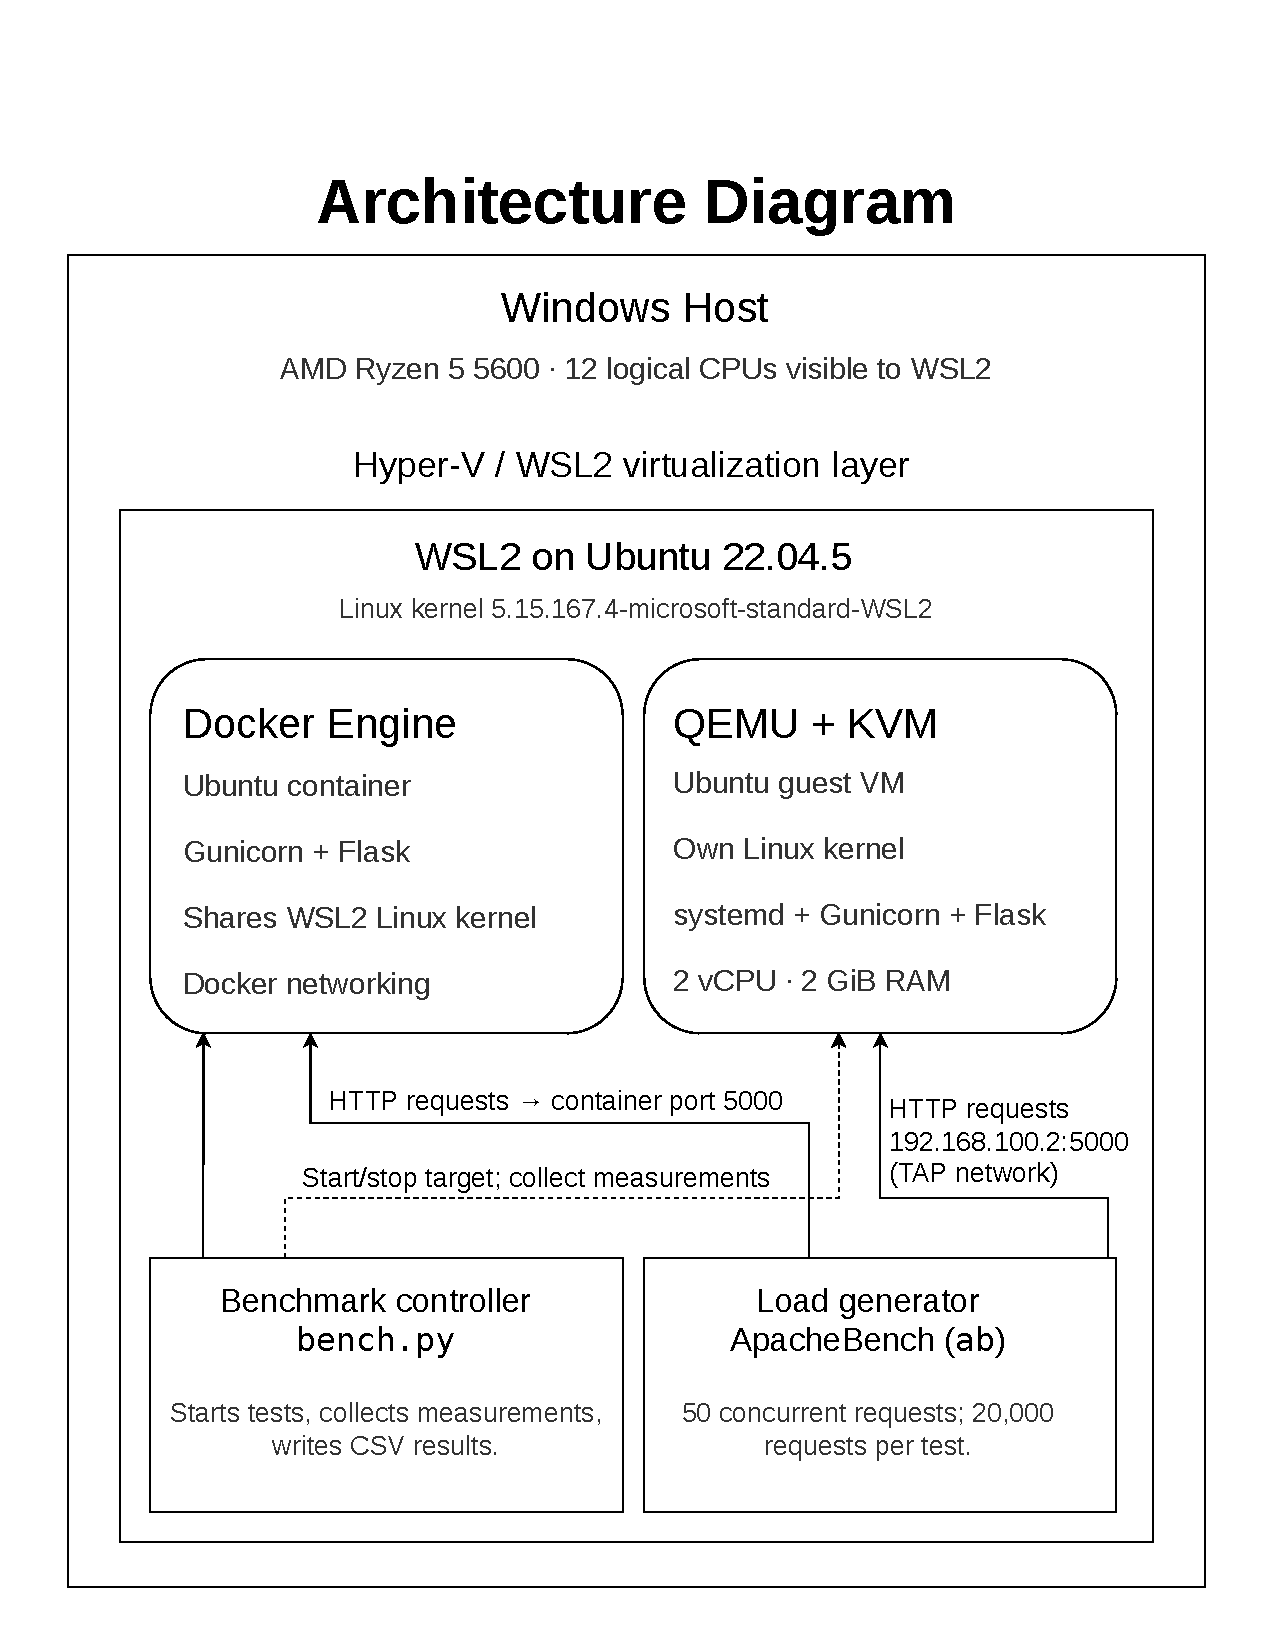
\includegraphics[width=0.9\linewidth]{figures/architecture.pdf}
    \caption{Architecture Diagram for the Docker container
    and QEMU/KVM virtual machine.}
    \label{fig:architecture}
\end{figure}

The data flow of a request is simply like this: The load generator opens a TCP connection from its selected cores. For the Virtual Machine, the packet crosses the TAP interface into QEMU and then is handled by the virtual network card. Then it’s delivered to the guest kernel, which gives it to Gunicorn, but for the container, the packet crosses the Docker bridge and virtual Ethernet pair. Then it’s delivered directly to the process in the container’s network namespace (restrictions). After this whole process, Gunicorn passes the request to one of the two Flask workers, and then the response is sent back within the same path. We’ve described both paths as it’ll help later on explain why the lightweight endpoint is sensitive to the target, more than the compute endpoint.

\subsection{Alternatives Compared}
This study doesn’t use any cloud provider, as the topic runs totally on a local machine. So, the cost is basically non-existent and doesn’t need to be taken into consideration, the only cost is the runtime of the machine itself which depends on the hardware of each setup and is minimal. We compare two alternatives, the first being \textbf{VM}: an Ubuntu 24.04 cloud image running under QEMU with KVM, using two virtual CPUs and two gigabytes of memory. The second is a \textbf{container} built on the \texttt{ubuntu:24.04} image, limited to the exact same budget of two cores and two gigabytes of memory. Since both use the same distro and version (Ubuntu 24.04) and application, the difference we measure focuses on the cost of virtualisation itself, and does not show the effect of base image choice. Smaller base images are usually used for containers as they’re better, like the Alpine, but that would be unfair for our comparison.

We used QEMU with KVM for the Virtual Machine because it’s open-source, and is scriptable from the command line which makes it easier for testing. IT also exposes the acceleration and networking options we need~\cite{b5}. We used Docker for hte container because it’s the most common container engine, and exposes cgroup limits directly~\cite{b4}. ApacheBench is also used for load, because it’s simple and available as a singular package, and gives us the throughput and latency percentiles in a format that makes it easy to parse and use~\cite{b6}. Python scripts automate the runs, and the analysis produces the tables and figures we’ve used in this paper directly from the generated CSV files. This is all done to ensure no human-error like accidental copying or oversight can happen.

A few choices done in this study require more context for justification. We chose two workloads because they put load on different parts of the system. The compute endpoint focuses on the processor time and would show delay cause by virtualisation on the CPU, and the tiny endpoint is more about the networking and would show the differences in request path. We chose two cores and two gigabytes of memory, a small but equal amount, because it’s enough to give the application the needed resources to run comfortably, while also leaving enough resources in the host for the load generator.

\subsection{Requirements and Responsibilities}
There are some requirements for this experiment. Your tested applications must have identical behavior in both options, and you must provide equal resources, and do repeated automated measurements. Table~\ref{tab:resp} lists who’s responsible for which layer, considering that this would be applied in a real cloud deployment split. For a Virtual Machine, the customer owns the guest kernel, and must also keep it updated. While the provider owns the hypervisor and hardware. For containers, the customer owns the image and the application, and the kernel belongs to the host owner and is shared by every container.

\begin{table}[htbp]
	\caption{Shared Responsibility: Virtual Machine versus Container (on a Cloud Provider's Infrastructure)}
	\begin{center}
		\footnotesize
		\begin{tabular}{|p{0.30\columnwidth}|p{0.27\columnwidth}|p{0.27\columnwidth}|}
			\hline
			\textbf{Layer} & \textbf{Virtual Machine} & \textbf{Container} \\
			\hline
			Physical hardware, hypervisor & Provider & Provider \\
			\hline
			Kernel and its patches & Customer (guest) & Host owner (shared) \\
			\hline
			User space and packages & Customer & Customer (image) \\
			\hline
			Isolation boundary & Hypervisor & Kernel namespaces \\
			\hline
			Application and data & Customer & Customer \\
			\hline
		\end{tabular}
		\label{tab:resp}
	\end{center}
\end{table}

\section{Methodology}
\label{sec:methodology}
\subsection{Environment}
I’ve listed the test environment in Table~\ref{tab:environment}. All measurements were made on a singular desktop computer using an AMD Ryzen 5600 processor (six cores, twelve logical CPUs), 32 GB of memory, running Ubuntu 22.04 in WSL2. The Virtual Machine and the container both use Ubuntu 24.04, and use up two cores and two gigabytes of memory. All the version numbers and records are taken from the environment file generated by the scripts.

\begin{table}[htbp]
	\caption{Experimental Environment}
	\begin{center}
		\footnotesize
		\begin{tabular}{|p{0.28\columnwidth}|p{0.62\columnwidth}|}
			\hline
			\textbf{Property} & \textbf{Value} \\
			\hline
			Host & AMD Ryzen 5 5600 (6 cores, 12 logical CPUs), 32 GB RAM; Windows 11 24H2 Build 26100 \\
			\hline
			WSL and Linux & WSL 2.3.26.0, Ubuntu 22.04.5, kernel 5.15.167.4 \\
			\hline
			Hypervisor & QEMU 6.2.0 with KVM, nested in WSL2; VM: 2 vCPUs, 2 GiB \\
			\hline
			Container engine & Docker 29.9.0, cgroup v1 \\
			\hline
			Guest / image OS & Ubuntu 24.04 LTS \\
			\hline
			Application & Flask 3.0.3, gunicorn 22.0.0, Python 3.10.12, 2 workers, 3 endpoints \\
			\hline
			Resource budget & 2 CPUs pinned to WSL2 logical CPUs 0--1, 2~GB \\
			\hline
			Load test tool & ApacheBench 2.3; 50 concurrent connections; 2 workloads \\
			\hline
			Load per run & 20000 requests per workload after a 500-request warm-up \\
			\hline
			Repetitions & 3 per configuration \\
			\hline
		\end{tabular}
		\label{tab:environment}
	\end{center}
\end{table}

\subsection{Launching the Two Implementations}
We started the Virtual Machine using with \texttt{qemu-system-x86\_64} with the options \texttt{-accel kvm}, \texttt{-cpu host}, two virtual CPUs, 2048 MB of memory, a virtio disk, and a virtio network device attached to a TAP interface. Every start gets a fresh copy on top of the prepared base image, so the states of each run don’t affect the runs after. The container on the other hand is run with \texttt{docker run} using \texttt{--memory 2g} and \texttt{--cpuset-cpus} for the same two cores, again as a fresh container each time.

The application is a Flask service by Gunicorn with two workers, with one worker assigned for each core. The \texttt{/health} endpoint returns a short message indicating that it succeeded, and is used just to check if it’s ready. The \texttt{/} endpoint returns a tiny response, so almost no application time is spent per request, and the \texttt{/compute} endpoint performs 5000 chained hash operations per request. This keeps the processor busy for a measurable time. All the data is synthetic, and both options run exactly the same code, from the exact same source file, so the measurements are not affected by difference in these.

I chose these metrics to match what the operating system cares about. The setup time checks out how quickly capacity appears, idle memory and disk check how many instances can fit on a host, and throughput and latency capture how well an instance can serve users. Using the 95th percentile instead of the maximum is important because a singular irregularity would affect the maximum, and this would change the standard deviation result which is important to keep proper as the guidelines ask for the average and spread of multiple or repeated runs.

\subsection{Measurements}
The setup time in this setup is the time from starting the container or Virtual Machine until \texttt{/health} returns HTTP 200. We do one warm-up round, then three measured runs in random order while also checking every 20~ms. We measure memory usage around 20 seconds after readiness, and for the Virtual Machine we measure QEMU’s memory and memory usage on the host. We check the container’s memory usage from \texttt{docker stats}. We also measure the Virtual Machine disk image’s allocated space and the Docker image size, and use ApacheBench with 50 concurrent connections and 20,000 requests. We made those tests on two workloads: \texttt{/compute}, which is the 5000 chained hash test, and \texttt{/}, which is a tiny response dominated by the network. We disable keep-alive so each request opens a new connection. All resources are local, so the cost (USD) in cash is nonexistent, zero.

\textbf{Expectations (written before measuring).} H1: the container is ready in less than or in an about a second, while the Virtual Machine needs several seconds, because it has to boot a kernel and a whole init system. H2: container memory is close to the application's own use, wheras the Virtual Machine requires running an additional Operating System on the guest. H3: processor bound throughput is very close to the original, because KVM runs the code on the hardware directly, and any gap comes from the network path and virtual devices, in line with~\cite{b3}.

To make sure that every start is used on a fresh copy or a fresh container, for the write disk, we reduced the noise and made the load generator run on separate cores. We were able to reduce the noise by giving both options the exact same CPU and memory, and set them to the same cores. Only one ran at a time, but the order of running them was randomised, and we didn’t take the warm-up round into consideration. We also waited for around 15 seconds between each test, and the background update services were disabled in the Virtual Machine so they don’t disturb the measurements. We also closed any other background apps from the local machine to have a completely interference-free environment to not affect any measurement taken.

We measured each configuration in three rounds (after discarding the warm-up round), and for every metric we mention the mean and the sample standard deviation over all three rounds, then we use the standard deviation as the spread. The throughput in this is the requests per second value, reported by ApacheBench, and the 95th percentile comes from the percentile table.

\subsection{Reproducibility and Verification}
All code is in the repository (Appendix~\ref{app:code}). All of the steps to build the Docker image, the Vitual Machine, running scripts, and so on, are properly listed in README. Raw \texttt{ab} outputs and CSV files are also included, so that every number in the tables put in this paper can be looked back at in source. Fig.~\ref{fig:shot1} shows the container being deployed and load tested. AI was used to help write the testing scripts and format the README, but the core logic was completely implemented by me while referring to the the relevant documentation, as it’s important to pay attention to efficiency and correct system behaviour to ensure that no real critical system error occurs.

\begin{figure}[htbp]
	\centering
	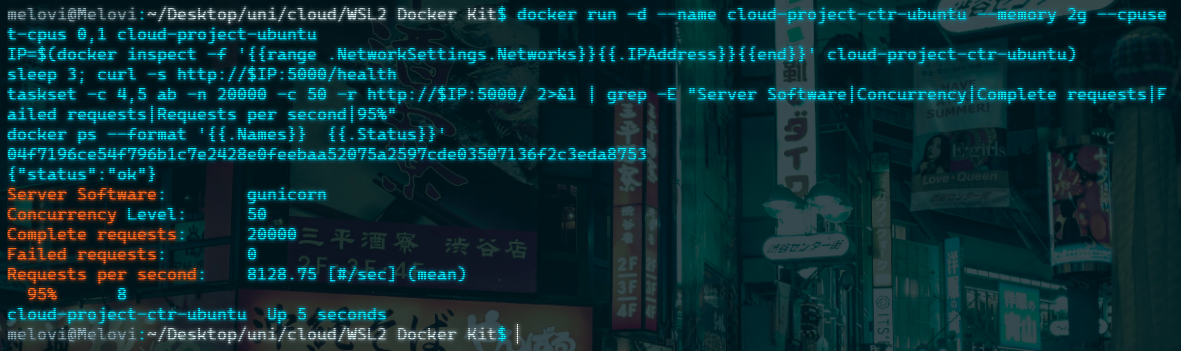
\includegraphics[width=0.95\columnwidth]{figures/shot1_container.png}
	\caption{Container deployment: \texttt{docker run}, health check, and the \texttt{ab} summary (20000 requests, no failures).}
	\label{fig:shot1}
\end{figure}

\section{Results}
\label{sec:results}
\subsection{Performance Results}
I’ve shown the startup and idle memory results in the Table~\ref{tab:startup} and Fig.~\ref{fig:startup}. The container is ready after ~0.77 seconds on average (standard deviation is ~0.03 seconds), while the Virtual Machine needed ~7.34 seconds (standard deviation is ~0.29 seconds). So the container basically started up around 9.5 times faster. The gap is incredibly large, in both cases: even the slowest container round was way quicker than the fastest Virtual Machine round. And idle memory shows a similar picture, as the container used around ~42 MB, whereas the QEMU used around ~522 MB on the host. The guest operating system seemed to show about ~353 MB in use, and that shows that the host side figure includes more than their own use, so the container figure is much lower. But the two numbers aren’t really measured in an identical way, there is a limitation later to be discussed.

\begin{table}[htbp]
	\caption{Time to Ready and Idle Memory (mean $\pm$ s.d.)}
	\begin{center}
		\footnotesize
		\resizebox{\columnwidth}{!}{\begin{tabular}{|l|c|c|c|c|}
\hline
\textbf{Target} & \textbf{Ready (s)} & \textbf{Host mem. (MB)} & \textbf{Guest mem. (MB)} & \textbf{n} \\
\hline
VM & 7.34 $\pm$ 0.29 & 522.1 $\pm$ 1.1 & 352.7 $\pm$ 10.4 & 3 \\
\hline
Ctr-Ubuntu & 0.77 $\pm$ 0.03 & 42.2 $\pm$ 0.1 & 42.2 $\pm$ 0.1 & 3 \\
\hline
\end{tabular}
}
		\label{tab:startup}
	\end{center}
\end{table}

\begin{figure}[htbp]
	\centerline{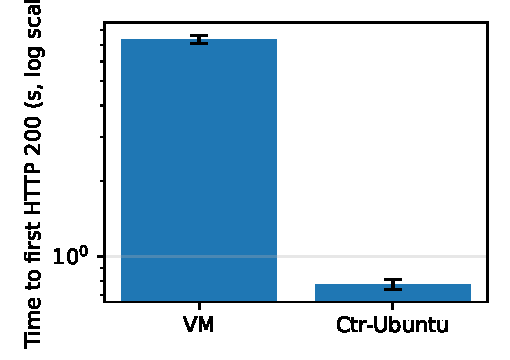
\includegraphics[width=0.8\columnwidth]{figures/fig_startup.pdf}}
	\caption{Time to first successful HTTP response after the start command (three rounds, error bars: one standard deviation, logarithmic axis).}
	\label{fig:startup}
\end{figure}

You can check the disk footprint in Table~\ref{tab:size}. The Virtual Machine image occupies around 2334 MiB, while the container image occupies around 212 MiB, which is around eleven times smaller. These two numbers (of memory) don’t really hold the same kind of data, the Virtual Machine figure is the allocated size of a QCOW2 disk that holds a full operating system, kernel, and boot files. While the container figure is merely the size of a Docker image made of layers that are on the host kernel, so it is naturally a lot more memory-efficient. We still report both because these are still important parameters, especially for those who care about storing and distribution and for operators.

\begin{table}[htbp]
	\caption{Disk Footprint}
	\begin{center}
		\footnotesize
		\begin{tabular}{|l|c|}
\hline
\textbf{Target} & \textbf{Size on disk (MB)} \\
\hline
VM & 2334 \\
\hline
Ctr-Ubuntu & 212 \\
\hline
\end{tabular}

		\label{tab:size}
	\end{center}
\end{table}

I’ve put the results for the processor bound \texttt{/compute} endpoint in Table~\ref{tab:sat_compute}. The container reached ~961 requests per second (standard deviation 69) compared to ~724 requests per second (standard deviation 10) for the Virtual Machine. This is around 33 percent higher, but the 95th percentile latency was around 68.7 ms for the container and 98 ms for the Virtual Machine. This shows that the container’s spread accross the runs was significantly larger than the Virtual Machine’s, so we shouldn’t read too mcuh into exact size of the gap with three runs even if it’s enough. Peak memory during load stayed at ~47 MB for the container, with a whopping ~913 MB for the Virtual Machine which is crazy higher.

\begin{table}[htbp]
	\caption{CPU-Bound Workload (\texttt{/compute}, 50 Connections, mean $\pm$ s.d. of 3 Runs)}
	\begin{center}
		\footnotesize
		\resizebox{\columnwidth}{!}{\begin{tabular}{|l|c|c|c|c|c|}
\hline
\textbf{Target} & \textbf{Req/s} & \textbf{Median (ms)} & \textbf{p95 (ms)} & \textbf{Peak mem. (MB)} & \textbf{n} \\
\hline
VM & 724 $\pm$ 10 & 60.7 $\pm$ 2.5 & 98.0 $\pm$ 6.1 & 913 $\pm$ 2 & 3 \\
\hline
Ctr-Ubuntu & 961 $\pm$ 69 & 48.0 $\pm$ 3.5 & 68.7 $\pm$ 11.1 & 47 $\pm$ 0 & 3 \\
\hline
\end{tabular}
}
		\label{tab:sat_compute}
	\end{center}
\end{table}

Now for the lightweight \texttt{/} endpoint shown in Table~\ref{tab:sat_index}, the gap is quite larger. The container served ~7481 requests per second (standard deviation 802) compared to ~3579 requests per second (standard deviation 270) for the Virtual Machine. Literally more than double, at 2.1 times the amount, and the 95th percentile latency was ~10.3 ms compared to ~20.7 ms. You can see the comparison of both workloads in Fig.~\ref{fig:load}. Because this endpoint does basically no computation, the result is mostly dominated by the network, which means that the path between the load generator and the target matters here, definitely more than the processor. All twelve test runs completed 20,000 requests and none of them failed.

\begin{table}[htbp]
	\caption{Network-Bound Workload (\texttt{/}, 50 Connections, mean $\pm$ s.d. of 3 Runs)}
	\begin{center}
		\footnotesize
		\resizebox{\columnwidth}{!}{\begin{tabular}{|l|c|c|c|c|c|}
\hline
\textbf{Target} & \textbf{Req/s} & \textbf{Median (ms)} & \textbf{p95 (ms)} & \textbf{Peak mem. (MB)} & \textbf{n} \\
\hline
VM & 3579 $\pm$ 270 & 13.7 $\pm$ 0.6 & 20.7 $\pm$ 1.5 & 912 $\pm$ 2 & 3 \\
\hline
Ctr-Ubuntu & 7481 $\pm$ 802 & 6.3 $\pm$ 0.6 & 10.3 $\pm$ 2.5 & 47 $\pm$ 0 & 3 \\
\hline
\end{tabular}
}
		\label{tab:sat_index}
	\end{center}
\end{table}

\begin{figure}[htbp]
	\centerline{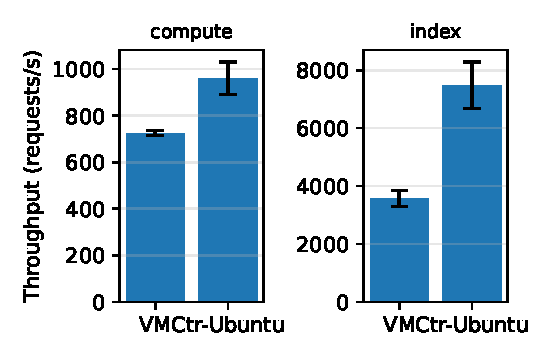
\includegraphics[width=0.9\columnwidth]{figures/fig_load.pdf}}
	\caption{Maximum throughput for the two workloads (50 concurrent connections, 20000 requests per run). Error bars: one standard deviation over three runs.}
	\label{fig:load}
\end{figure}

Seeing all of these loading results, we can tell that there are two different behaviours. When the endpoint is processor bound, both options spend most of their time computing hashes on the same two cores, and the gap basically shrinks to a small amount. But when the endpoint is almost empty, the cost of each request is dominated by accepting a connection, and basically just passing it through the network path and writing a response. Here, in the networking part, the gap grows to an even larger amount. The latency also seems to have the same pattern, where the median and 95th percentiles are both lower for the container on both endpoints.

About the startup time, since the container’s takes ~0.77 seconds, it means that a scale out decision can be put into action directly in less than a second. Whereas the Virtual Machine needs more than seven seconds under the same conditions. The container’s startup was also more consistent in general, regardless these numbers measure only the local start of an instance. Basically what it means is that it’s on a host that already exist, so it’s easier and they exclude image download, scheduling, and health check delays. Those are things that we should take into consideration, and the absolute values should not be copied directly.

\subsection{Cost Results}
The total cost for this study was 0 USD, since both implementations are ran locally no cloud service used. Of course, the cost of electricity and runtime of this local machine is not taken into consideration, or labor and production hosting. After the runs, I’ve executed the cleanup script and confirmed that everything I’ve setup was completely removed, such as the containers, images, and the Virtual Machine disk, they were all deleted and cleaned up with no sight. Fig.~\ref{fig:shot2} shows the empty leftover check.

\begin{figure}[htbp]
	\centering
	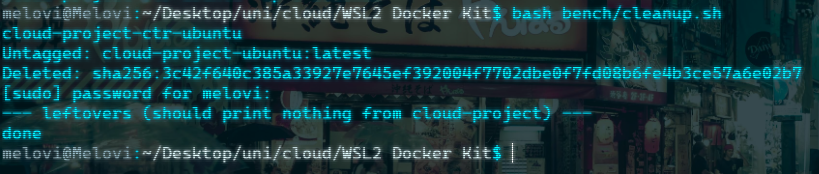
\includegraphics[width=0.95\columnwidth]{figures/shot2_cleanup.png}
	\caption{Cleanup confirmation: the leftover check printed by \texttt{cleanup.sh} is empty.}
	\label{fig:shot2}
\end{figure}

\subsection{Comparison of Alternatives}
There are other options out there that might make more sense than our setup, like they could’ve been run on a Linux machine instead of WSL2 for example. And that would avoid the extra virtualisation layer. Another hypervisor option we could’ve taken, and actually more popular, would be VirtualBox, or to test containers running inside a virtual machine. However, I’ve focused specifically and solely on comparing Docker containers with QEMU/KVM virtual machines inside WSL2 in this study. Simply, testing these other approached could be useful to see how much the environment affects the results, and this might prove useful to someone with these specific setup requirements.

You can see the direct comparison as a summary in the Table~\ref{tab:summary}. The container clearly wins on every measured evaluation in this setup, as its startup time is around 9.5 times faster, it uses around 12 times less memory, needs about 11 times less disk space, and serves more requests per second. Not to mention the lower latency on both of the workloads. And even though we didn’t find any section where the Virtual Machine would offer a performance benefit, its main thing is about having a separate kernel and stronger isolation boundary.

\begin{table}[htbp]
	\caption{Summary of Container versus VM (ratios from the mean values)}
	\begin{center}
		\footnotesize
		\begin{tabular}{|p{0.38\columnwidth}|c|c|c|}
			\hline
			\textbf{Metric} & \textbf{VM} & \textbf{Container} & \textbf{Ratio} \\
			\hline
			Time to ready (s) & 7.34 & 0.77 & 9.5$\times$ faster \\
			\hline
			Idle host memory (MB) & 522.1 & 42.2 & 12.4$\times$ less \\
			\hline
			Disk (MiB) & 2334 & 212 & 11.0$\times$ smaller \\
			\hline
			\texttt{/compute} (req/s) & 724 & 961 & 1.33$\times$ \\
			\hline
			\texttt{/} (req/s) & 3579 & 7481 & 2.09$\times$ \\
			\hline
		\end{tabular}
		\label{tab:summary}
	\end{center}
\end{table}

\section{Discussion}
\label{sec:discussion}
Based on the results, the obvious better choice for this environment is the container. The main difference is the startup time, and its explanation is simple. A container is a process started on a kernel that is already running, whereas the Virtual Machine must start QEMU first, boot a guest kernel, and run the init system before starting the application to later on answer the request~\cite{b2}. The same reason can be said for memory and disk, since the Virtual Machine carries a whole operating system, it uses a lot of memory for it. Whereas the container carries only user files, as well as the application. This matches our general expectations of those options, and is consistent with the near zero compute overhead of container reported by Felter et al.~\cite{b3}. In our scenario, QEMU launched in around 0.16 seconds, whereas the Virtual Machine launched in 7.34 seconds, so most of the delay was basically from the guest boot.

To answer the question of whether startup difference matters for autoscaling: our measurements showed an extra 6.60 seconds peer instance, that means that potentially a whole Virtual Machine based group of server would react to a spike literally several seconds later than a container based one, which might seem trivial but during that time requests are queued and piled up. For a service with a load that changes very slowly, this delay won’t matter that much, but if the service has a crazy amount of traffic that it can literally cause errors for users. In a real cloud, the Virtual Machine would also have to be placed on a host with a disk, so the real issue might not be revealed with our local measurement, it literally might be worse and the gap might be larger.

The results need careful reading, especially the throughput readings, as the processor bound endpoint has an understandable modest gap, and that fits the expectations as KVM executes code directly on the processor. But the lightweight endpoint doesn’t have much, and the container is about twice as fast. The Virtual Machine passes through more layers per request as it receives traffic through a TAP device with a virtual network card. Felter et al.\ says that virtualised networking is a main source of overhead~\cite{b3}. And this actually supports our findings, we can’t say that our work proves it but it definitely is consistent with his observations.

In terms of security, the Virtual Machine has a hypervisor, and the customer fixes up the guest kernel. In containers, they share the host kernel, so a kernel vulnerability could effect literally every container on the host, as seen in Table~\ref{tab:resp}. In both models, the customer is responsible for the application and related data, and this is why cloud providers commonly run containers of different customers inside separate Virtual Machines. This combines the fast startup of containers with the isolation of hypervisor (the main benefit that comes from using Virtual Machines, minus the delays).

The difference in disk, however, is substantial in a different sense, and it depends on what each option contains. The Virtual Machine holds a kernel, boot loader, system devices, a package etc. on top of the space allocated for the virtual disk. The container on the other hand only has the image itself and the user space layers for the application, as it relies only on the host kernel. Those image layers can also be shared between images within a host, kinda like caching. So running many containers from one image multiplies the memory use, but not the stored image, whereas in Virtual Machines it’ll need its own disk for every singular one. For a huge amount of instances, this really causes a big number and matters a lot.

The comparison would look different in the typical cloud deployment, as containers usually run inside Virtual Machines. So, the startup cost of the Virtual Machine is paid once per host, and not per container, which is how systems actually do fast scaling without having security constraints (hypervisor). The hypervisor would also be running on the hardware, instead of QEMU nested inside a WSL2 like what we did, which likely reduces the Virtual Machine overhead in our research. So we can say that our measurements are a comparison of these two implementations, not really a prediction for a managed cloud service, so this information would be highly specific.

There are some areas in this comparison that can be unfair, but they’re mostly subtle, but we still list how we tried to avoid them. We setup both targets to use the same Ubuntu version, same application, worker count, and resource budget (memory and cores). And both workers are pinned to the same cores, the system was also setup in a random manner, so there can’t be anything favoring the other. Some differences still exist, like the Virtual Machine has its own kernel and Virtual Devices, which makes it unfair as the container uses the host kernel. These are not flaws, definitely not of the test, but are actually the differences this study aims to measure as both have their own uses.

Our study also has several limitations, unfortunately. Everything runs inside WSL2, so the Virtual Machine is a nested one, and has an extra hidden layer. That is really the main limitation, but it’s also important to mention that the memory and disk figures are not exactly comparable, since the Virtual Machine memory includes the QEMU process, and the container memory comes from a cgroup counter, it would be two different allocations. The last limitation I can mention is that the tests were short, they’re not meant for large enterprises or corpos but rather for users who find themselves in specific situations alike, but they should still provide useful insight.

Since we measured each configuration only thee times, we can only provide rough estimates with these standard deviations, but the large gaps in startup time, memory, and disk are really outside of the spread, so we’re confident about their direction. The throughout gap on the processor bound endpoint is smaller, and container’s own spread is about seven percent of its mean, so the ratio of 1.33 should be treated as an approximation. More repetitions would’ve been ideal, especially if we had the chance to do something like repetition over several days, that would really boost the confidence of these results,. So the means should be taken with a grain of salt as they’re rough estimates.

Something to mention about the cost, even though I’ve mentioned that the cost was basically zero in cash, the results still show that we can save a lot in production. The container for example used ~42 MB of host memory compared to ~522 MB for the Virtual Machine, and around one tenth of disk space. This would’ve allowed more workloads to share the same resources, which would reduce costs by a crazy standard. For example, ten AWS EC2 instances at \$15.18 per month would’ve costed \$151.80, whereas containers sharing fewer instances could reduce that expense by a crazy amount (you can say 1 instance vs. 10).

Before running the tests within this experiment, I already expected the container to have a faster startup, and use fewer resources. The results confirmed both hypotheses I had, but the lightweight endpoint was a surprise, as the container achieved about 2.1 times the Virtual Machine’s throughput. I basically didn’t expect that networking overhead would matter this much.

I can give a reasonable recommendation based on our measurements, and the security considerations. That would be to choose the packaging by use case, for example: for stateless web services that need to quickly scale and have high traffic and be updated often, containers are better. This is mostly because instances have an incredible fast startup time (less than a second) and have low memory and disk usage. For workloads that require a different operating system or kernel for whatever reason, or stronger isolation, then Virtual Machines would be the better option. Though, not to anyone’s surprise, the best answer is to use both, and that is to have containers running inside Virtual Machines.

\section{Conclusion and Future Work}
\label{sec:conclusion}
In this specific setup, the container startup took ~0.77 seconds vs QEMU/KVM’s ~7.34 seconds, used about ~42 MB vs ~522 MB for the Virtual Machine. The Docker image was 212 MiB vs 2334 MiB for the Virtual Machine disk, and it served 33 percent more requests per second on the processor bound endpoint, and about 2 times the lightweight ones. Both setups had zero cost because everything was run locally, excluding the electricity and labor. Considering all of this, we recommend containers services that must scale quickly and have heavy usage in runs. The Virtual Machine remains the better choice where a separate kernel and stronger isolation are required, surely. These conclusions apply to this application specifically under nested WSL2, and this has been done under three measured runs so it should not be read as a universal ranking.

In this study, I’ve learned that the gap really depends on what we’re measuring. It’s large for startup, memory, and disk, but moderate for processor related work, apart from this though the actual main lesson is that fair comparison needs a lot of equal condition which is usually not possible. With more time we could repeat this experiment on a native Linux host or with VirtualBox instead of nested WSL2, and run more repetitions to have more confidence in the results, or test a container running inside a Virtual Machine which is how they’re usually deployed in the cloud, but with different standards.

\section*{AI Tool Use and Originality Declaration}
\label{sec:ai_declaration}
AI-assisted tools, mainly NotebookLM and Claude, were used to help develop and debug and structure benchmarking scripts, shape the README documentation, clarify technical concepts, and assist with LaTeX formatting. AI assistance also took part in some of the interpretation of results and costs. I configured and ran the experiments all by myself, and reviewed the reported measurements against the outputs of my own tests. I take responsibility for the accuracy, originality, reproducibility, and integrity of the final report and its contents.

\begin{table}[htbp]
	\caption{AI Use Disclosure Summary}
	\label{tab:ai_use}
	\centering
	\footnotesize
	\begin{tabular}{|p{0.30\linewidth}|c|p{0.44\linewidth}|}
		\hline
		\textbf{Project Stage} & \textbf{Level} & \textbf{Brief Description} \\
		\hline
		Topic and question & 0 & I chose the topic myself because I already use WSL2 and had learned about Docker and containers. \\
		\hline
		Literature and documentation search & 1 & I used AI for limited help understanding technical concepts and finding relevant documentation. \\
		\hline
		Design, deployment, and configuration & 3 & I used AI to help write and debug testing scripts, and setup specific configrations on the terminal alongside documentations. \\
		\hline
		Measurement, cost analysis, and modeling & 1 & I used AI to help compare the results based on other unfamiliar services. \\
		\hline
		Writing, editing, and LaTeX formatting & 2 & I used AI to help with LaTeX formatting, structuring tables, and checking how technical information was presented in the report. \\
		\hline
		Interpretation, discussion, and conclusion & 1 & I used AI for limited help explaining some of the technical results. \\
		\hline
	\end{tabular}
\end{table}

\begin{thebibliography}{00}

\bibitem{b1} P.~Mell and T.~Grance, ``The NIST definition of cloud computing,'' National Institute of Standards and Technology, Gaithersburg, MD, USA, NIST Special Publication 800-145, 2011. Available:
\url{https://csrc.nist.gov/pubs/sp/800/145/final}.

\bibitem{b2} J.~West, \textit{CompTIA Cloud+ Guide to Cloud Computing}, 2nd~ed. Boston, MA, USA: Cengage, 2024. Available:
\url{https://books.google.com/books/about/CompTIA_Cloud%2B_Guide_to_Cloud_Computing.html?id=ghrwzgEACAAJ&redir_esc=y}

\bibitem{b3} W.~Felter, A.~Ferreira, R.~Rajamony, and J.~Rubio, ``An updated performance comparison of virtual machines and Linux containers,'' in \textit{Proc. IEEE Int. Symp. Performance Analysis of Systems and Software (ISPASS)}, 2015, pp.~171--172. Available:
\url{https://explore.openaire.eu/search/publication?pid=10.1109%2Fispass.2015.7095802}

\bibitem{b4} Docker Inc., ``Resource constraints,'' Docker Docs. [Online]. Available: \url{https://docs.docker.com/engine/containers/resource_constraints/}.

\bibitem{b5} QEMU Project, ``System emulation,'' QEMU documentation. [Online]. Available: \url{https://www.qemu.org/docs/master/system/index.html}.

\bibitem{b6} Apache Software Foundation, ``ab - Apache HTTP server benchmarking tool,'' Apache HTTP Server Documentation. [Online]. Available: \url{https://httpd.apache.org/docs/current/programs/ab.html}.

\end{thebibliography}

\appendix

\section{Code Repository and Evidence}
\label{app:code}

Scripts and configuration files are available at: \url{https://github.com/Melovii/virtualisation-benchmark}

The repository contains the application and its two Dockerfiles (\texttt{app/}), the VM build scripts (\texttt{vm-qemu/}), the benchmark harness and analysis scripts (\texttt{bench/}), and the raw results (\texttt{results/}). No access keys, passwords, or private keys are included: the SSH key pair used to reach the VM is generated locally during the VM build and is excluded from version control.

Listing~\ref{lst:launch} shows the two launch commands used by the harness, with the same budget of two cores and two gigabytes for both targets. The VM starts from a fresh overlay disk on every start, and the container is removed and recreated every time.

\begin{lstlisting}[language=bash, caption={Launch commands used by the harness (simplified)}, label={lst:launch}]
# VM (TAP = tap device, overlay.qcow2 = fresh overlay)
taskset -c 0,1 qemu-system-x86_64 \
  -accel kvm -cpu host -machine q35 \
  -smp 2 -m 2048 \
  -drive file=overlay.qcow2,if=virtio \
  -netdev tap,id=n0,ifname=TAP,script=no \
  -device virtio-net-pci,netdev=n0 \
  -display none -daemonize
# Container (IMAGE = image name)
docker run -d --memory 2g \
  --cpuset-cpus 0,1 IMAGE
\end{lstlisting}

Listing~\ref{lst:runs} reproduces the full set of measurements, from building the images to cleanup (about 40--60 minutes unattended).

\begin{lstlisting}[language=bash, caption={Reproducing all measurements}, label={lst:runs}]
docker build -t cloud-project-ubuntu \
  -f app/Dockerfile.ubuntu app/
bash vm-qemu/create_vm.sh   # one time
bash vm-qemu/net_up.sh      # TAP network
bash bench/run_quick.sh     # all measurements
bash bench/cleanup.sh       # remove everything
\end{lstlisting}

\end{document}
